\chapter{Realisatie}

% detailontwerp met bijbehorende berekeningen (voedingsstromen, waarden van
% componenten); aansluitschema's van kabels en connectors; detailschema’s van
% de hardware en listings van de software worden in de bijlagen opgenomen

\section{Software}
\label{sec:softreal}
Om de juiste data uit een frame te halen is er de nodige filtering nodig.
Het ontwerpen van deze filters doen we middels de stappen in het vision ontwerp.
Hieronder staat beschreven hoe het geïmplementeerd is, van frame acquisitie tot
I/O aansturing.

\subsection{Acquisitie}
\label{sub:acqreal}
%To you Ramon

\subsection{Kleuren filter}
\label{sub:kleurfilt}
Het filteren van de kleuren moet zo snel mogelijk gebeuren omdat het verwerken van 
RGB plaatjes erg zwaar is. De kleuren filter zelf is dan ook zo eenvoudig mogelijk 
geimplementeerd. Hieronder is wiskundig te zien hoe er van een RGB plaatje een 
grijswaarde wordt gemaakt.

$gr(x, y)[0 -> 255] = r(x, y) - (g(x, y) + b(x, y))$

Waarbij $gr$ de grijswaarde van de pixel is;
$r$ de rode waarde van de pixel;
$g$ de groene waarde van de pixel;
$b$ de blauwe waarde van de pixel;
$x$ de x positie van de pixel;
$y$ de y positie van de pixel.

\subsection{Contrast stretch}
\label{sub:contstr}
Om een betrouwbaardere threshold te kunnen maken gebruiken we een contrast stretch
operatie. Deze functie bepaald de laagste en hoogste waarde in het beeld en smeert
deze uit over het complete grijswaarde gebied.

Door een vermenigvuldigingsfactor te bepalen is het eenvoudig om dit te bereiken. De 
vermenigvuldigingsfactor zal uiteraard > 1 moeten zijn, maar kan ook een komma getal
zijn. Float operaties zijn dus essentieel en daarbij is een FPU (Floating Point Unit)
erg handig. Om de zware calculaties te verminderen wordt er gebruik gemaakt van een
LUT (Look Up Table) die hetzelfde bereik heeft als de grijswaarde. Gezien er gebruik
wordt gemaakt van een grijswaarde bereik van 256 moet de calculatie 256x worden
uitgevoerd.

De verhouding wordt als volgt bepaald:
$R = \frac{D}{Max - Min}$
Waarbij R de vermenigvuldigingsfactor is;
D het grijswaarde bereik;
Max de maximale pixel waarde in het originele beeld;
Min de minimale pixel waarde in het originele beeld.

Daarna kan de LUT gevuld worden:

\begin{cppcode}
value = i * R;
if value > D then value = D
lut[i] = value;
\end{cppcode}

Tot slot kan er eenvoudig vanuit de huidige waarde in de LUT de nieuwe pixel waarde
worden opgevraagd. Dit wordt over het hele beeld gedaan om een verbeterd contrast te
krijgen.

\subsection{Threshold}
\label{sub:threshold}
Als image threshold wordt er gebruik gemaakt van de ISO data variant. Dit is een
automatische threshold die de juiste waarde bepaald vanuit het histogram. Hierbij
wordt uitgegaan van een 2-piek verdeling tussen de achtergrond en object pixels.
Hierbij wordt gezocht naar een \emph{valley} van het histogram.

\begin{figure}
    \begin{center}
        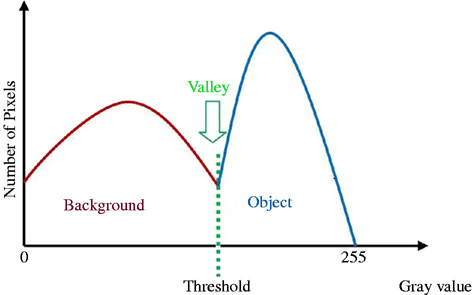
\includegraphics[scale=0.35]{figures/histogram.png}
    \end{center}
    \caption{Een 2-piek beeld verdeeld histogram}
    \label{fig:histogram}
\end{figure}

Vervolgens zal de functie van alle pixels boven/onder zijn threshold een 1 maken
en van alle pixels onder/boven zijn threshold een 0 maken.

De ISO data threshold gebruikt de 1ste pixel waarde en de som van alle pixels om
de threshold waarden te bepalen.
Wiskundig kan dat als volgt uitgedrukt worden:
$Th = s + \frac{\sum\limits_{x=0}^{x_max-1} \sum\limits_{y=0}^{y_max-1} f(x, y)}{x_max x y_max}  $
Waarbij $Th$ de threshold functie is;
$s$ de start waarde van de pixels.

Door de som van alle pixels tegelijk te bepalen met het histogram is het mogelijk
om een threshold te volbrengen na 2x het hele plaatje te hebben gescand.

In pseudo code zal dan de threshold waarde als volgt bepaald worden:

\begin{cppcode}
    for(i = 0; histogram[i] > 0; i++){
        i = i; //Do nothing
    }

    Th = i + (som / imageSize);
\end{cppcode}

Daarna  kan er eenvoudig met een if-statement een threshold worden gedaan:

\begin{cppcode}
    if(srcData >= min && srcData <= max){
        srcData = 1;
    } else {
        srcData = 0;
    }
\end{cppcode}

Gezien x en y waarden niet belangrijk zijn kan er het snelst door het plaatje
gegaan worden middels een pointer.

\subsection{Remove border blobs}
\label{sub:rembb}

Op het moment dat er een beeld binnen komt beschouwen we rand objecten als
nutteloos. Simpelweg omdat het niet zeker is wat het voor object is. Daarom
wordt er gebruik gemaakt van de "remove border blobs" operatie.

Er komt een binair plaatje binnen bestaande uit 1-en en 0-en. Door de 1-en
aan de rand van het plaatje te markeren met een ander nummer kan er een
border blob geïdentificeerd worden.

\begin{figure}
    \begin{center}
        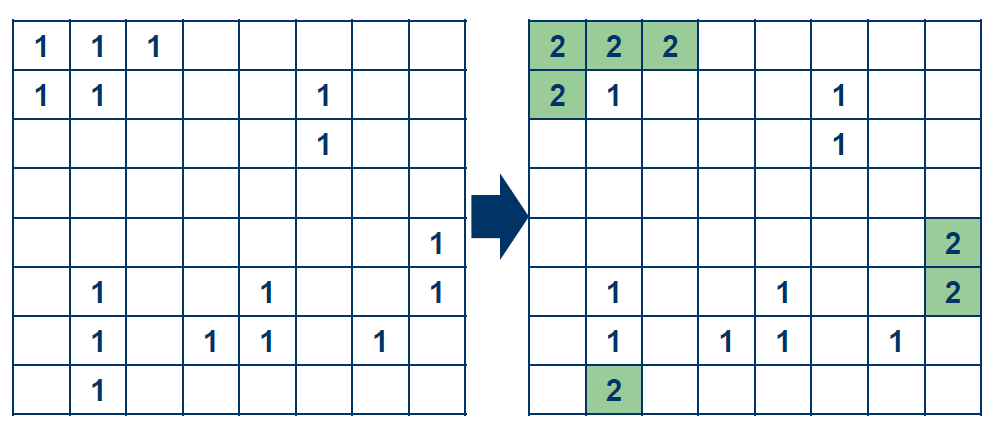
\includegraphics[scale=0.5]{figures/border_blob_step1.png}
    \end{center}
    \caption{Rand blobs markeren}
    \label{fig:bbstep1}
\end{figure}

Omdat enkel de rand gescand hoeft te worden kan deze functie redelijk snel
uitgevoerd worden.


\begin{cppcode}
for(w = width; w >= 0; w--){
	dst->data[0][w]      = dst->data[0][w] * 2;
	dst->data[height][w] = dst->data[height][w] * 2;
}
\end{cppcode}

Dit kan uiteraard ook eenvoudig voor de hoogte worden gedaan.

Het voltooien van het markeren is mogelijk door, als er een 1 gezien wordt,
te kijken naar de buren van deze pixel. Als dat een 2 is, dan mag deze pixel
ook gemarkeerd worden als een 2 enzovoort. Dit markeren kan van rechts-onder
naar links-boven en van links-boven naar rechts-onder gedaan worden om het
aantal iteraties te verminderen. Door iedere keer na een markeer ronde te
controleren of er een 1-2 verbinding bij x connected is, kan er bepaald worden
of er nog een keer over het plaatje gegaan moet worden om de overige pixels te
markeren.

\begin{figure}
    \begin{center}
        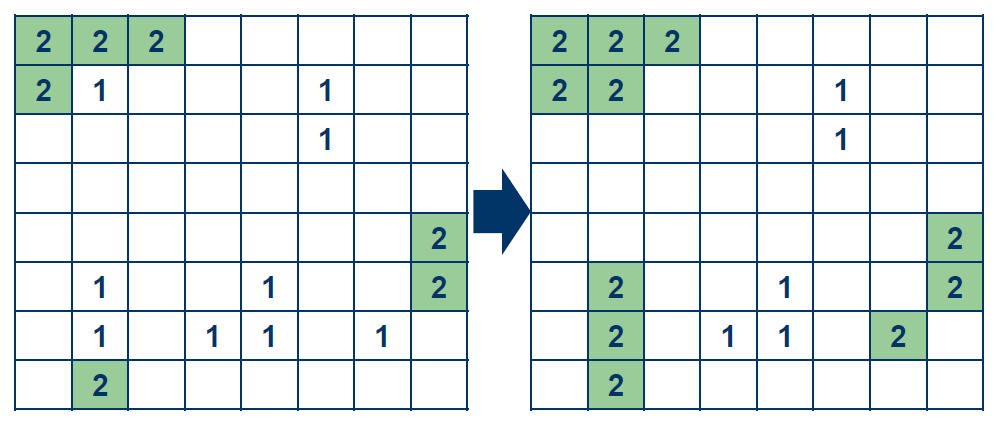
\includegraphics[scale=0.5]{figures/border_blob_step2.png}
    \end{center}
    \caption{Blijf scannen en markeren tot alles is gemarkeerd}
    \label{fig:bbstep2}
\end{figure}

De scan van links boven -> rechts onder en van rechts onder -> rechts boven
kan in 1 loop uitgevoerd worden.

\begin{cppcode}
//Lower right -> top left
if(img[i] == 1){
    if(iNeighbourCount(img, w, h, 2, connected) > 0){
        img[i] = 2;
    }
}

//Top left -> lower right
if(img[size - i] == 1){
    if(iNeighbourCount(img, (width - w), (height - h), 2, connected) > 0){
        img[size - i] = 2;
    }
}
\end{cppcode}

Tot slot kan er dan met een functie alle pixels met een 2 markeren als een 0.

\begin{figure}
    \begin{center}
        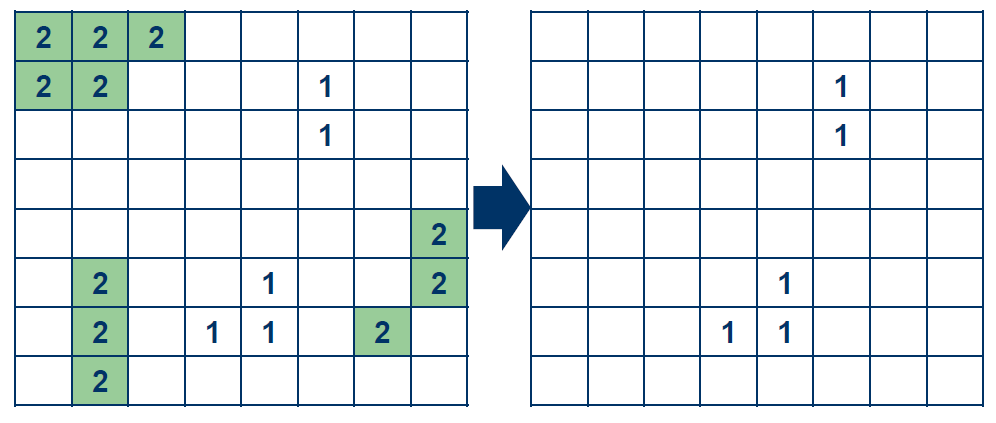
\includegraphics[scale=0.5]{figures/border_blob_step3.png}
    \end{center}
    \caption{Markeer alle 2-en als 0-en}
    \label{fig:bbstep3}
\end{figure}


\begin{cppcode}
if(img[i] == 2){
    img[i] = 0;
}
\end{cppcode}

\subsection{Fill holes}
\label{sub:fillholes}
Om betrouwbaar een object te kunnen identificeren vullen we de gaten op in de
objecten. Deze gaten kunnen ontstaan zijn bij de RGB filtering door schittering
op het object.

Het proces om de gaten te vullen is relatief eenvoudig. Door de achtergrond te
markeren en vervolgens alle niet gemarkeerde pixels op 1 te zetten is het vullen
voltooid.

Om een start te maken voor het markeren van de achtergrond is het mogelijk om
alle rand pixels die 0 zijn te markeren als, bijvoorbeeld, een 2. Dit zal op een
zelfde wijze gaan als bij de remove border blobs operator.

\begin{figure}
    \begin{center}
        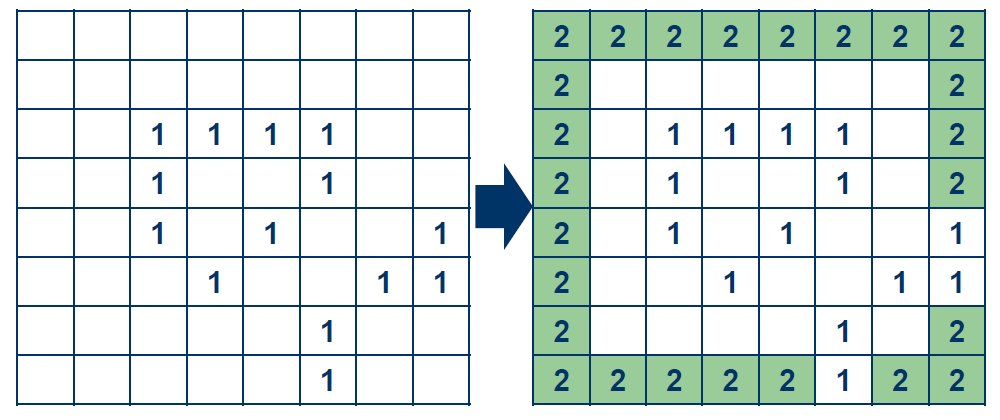
\includegraphics[scale=0.5]{figures/fill_holes_step1.png}
    \end{center}
    \caption{Achtergrond rand markeren.}
    \label{fig:fhstep1}
\end{figure}

Omdat enkel de rand gescand hoeft te worden kan deze functie redelijk snel
uitgevoerd worden.

\begin{cppcode}
for(w = width; w >= 0; w--){
	if(imgArr[0][w] == 0){
        imgArr[0][w] = 2;
    }
    if(imgArr[height][w] == 0){
        imgArr[height][w] = 2;
    }
}
\end{cppcode}
Dit kan uiteraard ook eenvoudig voor de hoogte worden gedaan.

Het voltooien van de pixel scan wordt op dezelfde manier gedaan als beschreven
bij de remove border blobs operatie. Vanuit alle gemarkeerde pixels wordt er
voortborduurt tot het hele plaatje is gemarkeerd. In dit geval mag er dus geen
2-0 bij x connected overgang meer zijn.

\begin{figure}
    \begin{center}
        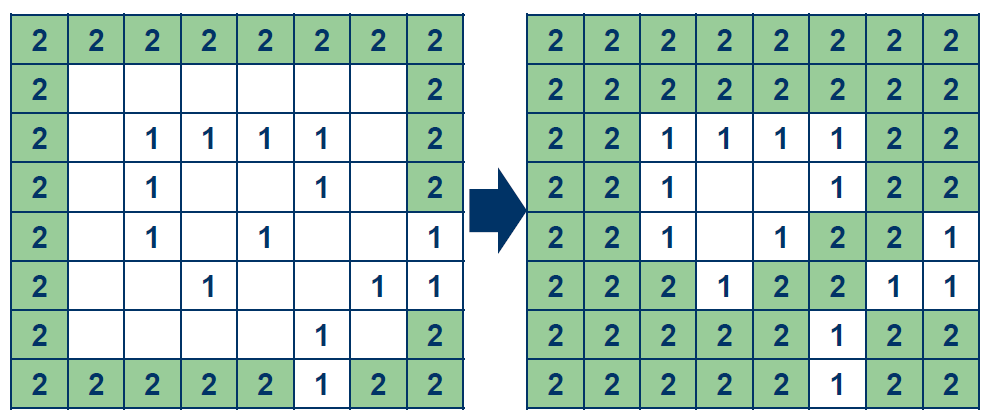
\includegraphics[scale=0.5]{figures/fill_holes_step2.png}
    \end{center}
    \caption{Achtergrond rand markeren.}
    \label{fig:fhstep2}
\end{figure}

Tot slot moeten alle 0-en gemarkeerd worden als een 1. Daarna mogen de 2-en
weer gemarkeerd worden als een 0. Helaas gaat dit niet in 1 stap omdat anders
het hele plaatje 1-en krijgt.

\begin{figure}
    \begin{center}
        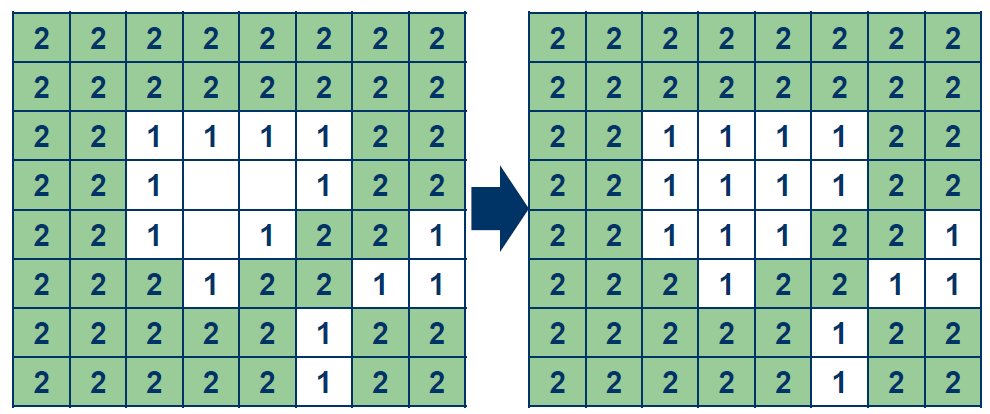
\includegraphics[scale=0.5]{figures/fill_holes_step3.png}
    \end{center}
    \caption{Blobs inkleuren.}
    \label{fig:fhstep3}
\end{figure}

\begin{figure}
    \begin{center}
        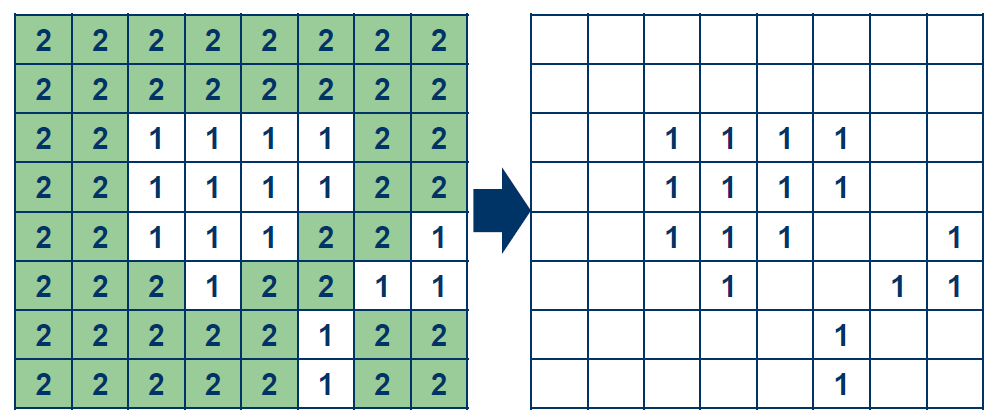
\includegraphics[scale=0.5]{figures/fill_holes_step4.png}
    \end{center}
    \caption{Achtergrond weer 0 maken.}
    \label{fig:fhstep4}
\end{figure}

\subsection{Label blobs}
\label{sec:labelblobs}
Om het benodigde object te detecteren is het nodig om ieder object te
identificeren. De makkelijkste manier om dit te doen is door ieder object een
nummer te geven. Zo kunnen van alle nummers de eigenschappen bepaald worden.

Deze operator is het meest complex en heeft dus ook de meeste tijd nodig.
Gelukkig is er voldoende ruimte voor snelheidsverbetering.

Door er voor te zorgen dat alle blobs een maximale waarde hebben kan er voorkomen
worden dat er nummer conflicten optreden. Daarvoor is het dus belangrijk eerst
alle pixels op 255 te zetten.

Vervolgens moet iedere pixel van 255 een nummer krijgen. Door het plaatje van
links boven -> rechts onder te doorlopen worden de blobs gelabeld. Door bij
iedere pixel te controleren of ze al een gelabelde pixel buur-pixel hebben
probeert het programma te voorkomen dat 1 blob 2 labels krijgt. Helaas is dit
niet helemaal te voorkomen. Kijk bijvoorbeeld naar onderstaand plaatje.

\begin{figure}
    \begin{center}
        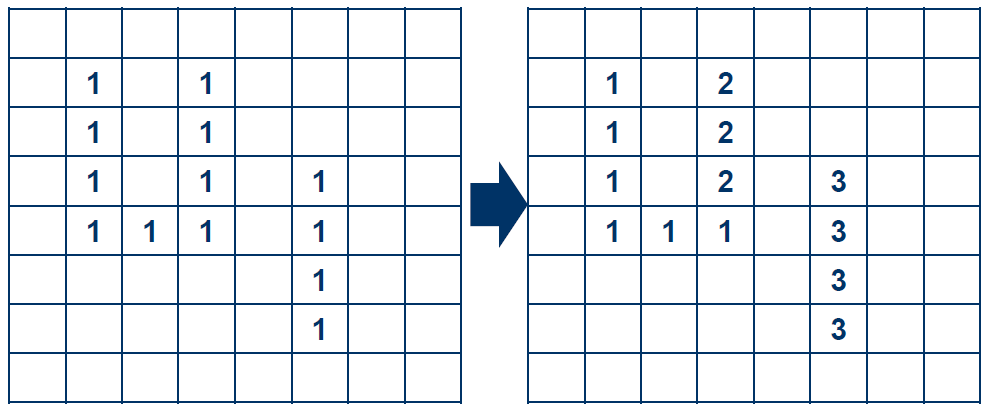
\includegraphics[scale=0.4]{figures/label_blobs_step1.png}
    \end{center}
    \caption{Verkeerd gelabelde blobs na de 1ste iteratie.}
    \label{fig:lbstep1}
\end{figure}

Het eerste label proces redelijk complex gezien er gekeken moet worden of een
blob al gelabeld is met een lager nummer ondanks dat al meerdere blobs gelabeld
zijn.

\begin{cppcode}
//If this pixel has to be labled
if(imgArr[h][w] == 255){
  blobDetected = 1;
  if(iNeighbourCount(img, w, h, blobCount, connected) > 0){ //If this blob is labeled
      imgArr[h][w] = blobCount;
  } else { //This blob might be labeled with a lower number or is a new blob
      for(j = blobCount; j != 0; j--){ //Check what number the neighbour might be
          if(iNeighbourCount(img, w, h, j, connected) > 0){
              foundFlag = 1;
              break;
          }
      }

      if(foundFlag){ //If this pixel is part of a labeled blob, set the right number
          imgArr[h][w] = j;
          foundFlag = 0;
      } else { //Otherwise, label this as a new blob
          blobCount += 1;
          imgArr[h][w] = blobCount;
      }

  }
}
\end{cppcode}
blobDetected wordt gebruikt als controle of er überhaupt wel een blob in het
plaatje is. Zo niet, dan kan er na deze iteratie ook gestopt worden met de
functie.

Vervolgens dient de dubbel gelabelde 1 label te krijgen. Dit is te bereiken
door te beginnen in de rechter onder hoek en zo naar links boven te werken.
Door iedere keer te kijken naar de pixels achter en onder het huidige pixel
kan de laagste waarde van de pixel worden bepaald. Het is uiteraard wel
belangrijk om rekening te houden met het x connected verhaal.
Daarna wordt hetzelfde gedaan alleen dan van de linker boven hoek naar de
rechter onder hoek. En tot slot wordt er gecontroleerd of alle blobs nu
maar 1 label hebben, zo niet, dan herhaalt het proces zich nog eens.

\begin{figure}
    \begin{center}
        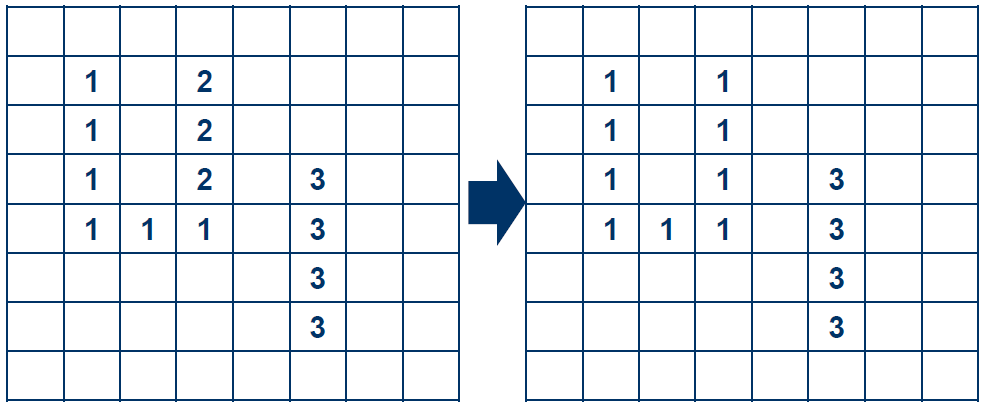
\includegraphics[scale=0.4]{figures/label_blobs_step2.png}
    \end{center}
    \caption{Uniform gelabelde blobs na (verschillende) iteraties.}
    \label{fig:lbstep2}
\end{figure}

Nu zijn er alleen gaten in de nummering. Dit kan opgelost worden door nog
één keer vaker over het plaatje te gaan en de blobs te labelen van links
boven naar rechts onder. Door een teller bij te houden kunnen de correct
gelabelde blobs automatisch worden genegeerd.

\subsection{Blob analyse}
\label{sub:blobanalyse}
Na het labelen kunnen de gevonden blobs/objecten worden geanalyseerd. Door
te controleren op massa/grootte van de blob bepaald het systeem waar het op
moet richten. Hierbij wordt de blob met de grootste massa genomen.

Eerst wordt er bij iedere blob bekeken wat de massa is van de blob.

\begin{cppcode}
//First clear the blob_mass registers
for(i = MAX_BLOB_COUNT; i > 0; i--){
    blob_mass[i] = 0;
}

for(i = (FRAME_SIZE - 1); i >= 0; i--){
    if(img[i] > 0){
        blob_mass[img[i]]++;
    }
}
\end{cppcode}

Dan wordt de grootste blob bepaald.

\begin{cppcode}
largest_blob = 0;

for(i = blobCount; i > 0; i--){
    if(blob_mass[i] > largest_blob){
        largest_blob = blob_mass[i];
    }
}
\end{cppcode}

Tot slot moeten de coördinaten van het middelpunt bepaald worden.

\begin{cppcode}
if(imgArr[h][w] == largest_blob){
    //Calculate height
    if(h < min_height){
        min_height = h;
    }
    if(h > max_height){
        max_height = h;
    }
    blob_pos_x = (max_height - min_height) / 2;

    //Calculate width
    if(w < min_width){
        min_width = w;
    }
    if(w > max_width){
        max_width = w;
    }
    blob_pos_y = (max_width - min_width) / 2;
}
\end{cppcode}

Met deze informatie kan de correctie bepaald worden.

\subsection{Calculate offset}
\label{sub:calcoffset}
% To you Ramon


\subsection{Pan \& Tilt controller}
\label{sub:panTiltContr}
De pan \& tilt controller zorgt er voor dat de servo.c file met de juiste outputs
wordt bestuurd met de juiste waarden. De servo.c file stuurt op zijn beurt de pwm.c
file aan met de juiste frequentie en Duty-Cycles (zet de hoek om in de juiste
Duty-Cycle). De pwm.c file zorgt er voor dat alle data naar de juiste file wordt
gestuurd, outputs niet dubbel geconfigureerd zijn etc..

Om een PWM signaal te genereren dient de PWM module geactiveerd te worden. Hoe
dit kan in Angström staat hieronder. Het voorbeeld is voor pin P8.13.

\begin{cppcode}
echo am33xx_pwm > /sys/devices/bone_capemgr.8/slots
echo bone_pwm_P8_13 > /sys/devices/bone_capemgr.8/slots
echo 20000000 > /sys/devices/ocp.2/pwm_test_P8_13.15/period
echo 10000000 > /sys/devices/ocp.2/pwm_test_P8_13.15/duty
\end{cppcode}

% Bron: http://www.phys-x.org/rbots/index.php?option=com_content&view=article&id=106:lesson-3-beaglebone-black-pwm&catid=46:beaglebone-black&Itemid=81

Zorg er wel voor dat de pinmode op PWM ingesteld staat. Dit kan worden gedaan
middels een overlay. Meer hier over in GPIO controller.

De \texttt{am33xx\_pwm} en \texttt{bone\_pwm\_P8\_13} kunnen standaard in slots worden gezet. Dit kan
bereikt worden door in uEnv.txt het volgende te zetten:
\texttt{capemgr.enable\_partno=am33xx\_pwm,bone\_pwm\_P8\_13}
uEnv.txt bevind zich op de virtuele SD kaart die automatisch verbind met de PC
tijdens het booten.

De period en duty tijd worden ingesteld via de pwm.c file. Daarnaast bouwt deze op
basis van het GPIO nummer automatisch de juiste directory op. Het enige wat
soms verandert is het suffix nummer van de directory (P8\_13.xx/). Dit kan echter
aangepast worden in de pwm.c file.

\subsection{GPIO controller}
\label{sub:gpiocontr}
Om GPIO's aan te sturen op de Beagle Bone Black dient de modus ingesteld te worden
samen met PULL-UP/PULL-DOWN weerstanden. Daarnaast dienen deze na iedere re-boot
weer ge-exporteert te worden om vervolgens te bepalen of het een input/output moet
zijn en om de waarde van de GPIO te wijzigen.

Het instellen van de pin modus en PULL-UP en PULL-DOWN weerstanden dient gedaan te
worden in de overlay. Dit is een .dts file waarin het volgende staat.

\begin{cppcode}
/* <Pin offset adres> <Value> </* pin comment */>*/
          0x0c0        0x07    /* 78: OUTPUT MODE7 + PULL-DOWN = Missile 1     */
\end{cppcode}

De waarden en pin offsets kunnen uit de tabellen in bijlage x gehaald worden. Hier
moet dus ook een PWM pin ingesteld worden indien deze nodig is!

Vervolgens dient de .dts file gecompileerd te worden naar .dtbo. Hieronder is het
commando te vinden er vanuit gaande dat de .dts file DM-GPIO-Test.dts heet.

\begin{cppcode}
dtc -O dtb -o DM-GPIO-Test-00A0.dtbo -b 0 -@ DM-GPIO-Test.dts
\end{cppcode}

Deze .dtbo file dient vervolgens gekopieerd te worden naar de /lib/fimware folder.
Om deze te activeren is er een re-boot nodig en vervolgens het volgende commando.

\begin{cppcode}
echo DM-GPIO-Test > /sys/devices/bone_capemgr.8/slots
\end{cppcode}

Uiteraard kan ook dit automatisch bij het opstarten gebeuren door deze in de
uEnv.txt file te zetten. Bij Pan \& Tilt controller staat hoe dit moet.

Om een GPIO te kunnen gebruiken dienen de volgende commando's uitgevoerd te worden.
Deze commmando's worden dan ook afgehandeld door de gpio.c file.

\begin{cppcode}
echo 60 > /sys/class/gpio/export
echo out > /sys/class/gpio/gpio60/direction
echo 1 > /sys/class/gpio/gpio60/value
\begin{cppcode}

Dit maakt de uitgang op GPIO 60 hoog. Laag is natuurlijk eenvoudig te realiseren
door 0 naar value te schrijven.
Het gebruik maken van een input is eenvoudig door \emph{in} naar direction te schrijven.
Dan is de waarde uit te lezen in value.

Als het programma afsluit is het netjes om de GPIO's ook weer te \emph{unexporten}.

\begin{cppcode}
echo 60 > /sys/class/gpio/unexport
\end{cppcode}

% Bron: http://derekmolloy.ie/beaglebone/beaglebone-gpio-programming-on-arm-embedded-linux/

\section{Hardware}
\label{sec:hardware}
Het lanceer systeem met camera wordt op een platform van hout (lasergesneder) 
gemonteerd. Dit betekend dat er 10 lucht slangen, een camera kabel en tilt servo 
kabel als bundel naar het platform worden geleid. De lucht kleppen zijn op het 
lanceer platform geplaatst, waardoor de lucht slangen een geringe lengte hebben.

\subsection{Shot control}
\label{sub:shotContr}
De shot control is een array van 10 MOSFETs die minimaal 1A kunnen schakelen ter behoeve 
van de inschakelstroom van de kleppen. Daarnaast dient er een blusdiode bij of in te 
zitten om de uitschakel piek te dempen. Een extern signaal zorgt er voor dat de kleppen 
een bepaalde tijd open blijven of kan zorgen zelfs voor een Rapid Boost™ lancering.

\subsection{Tilt control}
\label{sub:tiltContr}
Tilt control wordt gestuurd door een servo motor die met een arm aan het lanceer 
compartiment wordt bevestigd. De servo wordt bedient vanuit de BeagleBone Black die een 
uitgangssignaal van 0 - 3,3V heeft. Omdat de servo's een PWM signaal van 0 - 5V nodig 
hebben wordt er gebruik gemaakt van een transistor + pull-up weerstand. Zo wordt het 
signaal netjes om gezet naar 0 - 3,3V.

\subsection{Pan control}
\label{sub:panContr}
Pan control wordt ook gestuurd via een servo. Het pan platform wordt direct op de servo 
gemonteerd. Ook deze servo krijgt een PWM signaal via de BeagleBone Black. Deze wordt 
via dezelfde transistor schakeling aangestuurd.

\subsection{CPU}
\label{sub:cpu}
De CPU is in dit geval de BeagleBone Black. Dit is een out-of-the-box linux ontwikkelings 
bordje waar direct een USB camera op kan worden aangesloten en de nodige IO's.

\subsection{Veiligheid}
\label{sub:veiligheid}
Om onverwachts schieten te voorkomen wordt er gebruik gemaakt van een hardware beveiliging. 
Er is gekozen voor een beveiliging in hardware omdat dit het meest betrouwbaar is. Dit is 
geimplementeerd middels een D-type flip-flop die met een knop in- en uitgeschakeld kan 
worden. Deze flip-flop schakelt alle MOSFETs voor de kleppen uit en de pan/tilt servo's. 
Daarnaast wordt deze flip-flop uitgeschakeld vanuit het systeem als alle missiles op zijn. 
Er dient dan via een knop aangegeven te worden dat hij weer vol zit. Dan zal het systeem 
ook weer worden ingeschakeld.

Verder is er ook rekening gehouden met het feit dat, als de applicatie niet draait, er wel 
spanning op de outputs kan staan. Om te voorkomen dat er daardoor per ongeluk wordt geschoten 
boot de BeagleBone Black standaard met pull-down weerstanden op de juiste pinnen.

\subsection{Behuizing}
\label{sub:behuizing}
De behuizing van het systeem wordt een 10-stage raket lanceer station. Iedere stage krijgt dus 1
buisje ter behoeve van de luchtdruk. Er kunnen dus maximaal 10 schoten worden gelost voor er
herladen dient te worden.

\subsubsection{Launcher}
\label{subsub:launcher}
De zo genaamde launcher is het beweegbare compartiment waar alle Nerf darts in worden geladen
om af te schieten. Deze richt ook op de persoon.
De servo voor het tilt systeem wordt op het pan platform gemonteerd en met een arm aan de
launcher bevestigd. Dit wordt gedaan om de last op de servo te verminderen en de respons van
het systeem dus beter te maken. Ook wordt er aanbevolen om het scharnierpunt niet helemaal
achteraan te leggen zodat er een contragewicht is om nog meer last van de servo te halen.
Om het juiste montage punt van de arm van de servo te bepalen is er een serie driehoek berekeningen
nodig. Daarnaast kan er middels deze berekeningen ook de hoogte worden bepaald ten
opzichte van het pan platform (in verband met de neerwaartse beweging van het contragewicht).
Figuur 4.5 toont een schematische weergave van het systeem. In deze figuur is $S_1$ de lengte van
het scharnierpunt tot de voorkant, $S_2$ is de lengte van het scharnierpunt tot de achterkant. $\alpha$ geeft
de maximale hoek aan van de launcher en $\delta/B$ is de uitslag van de achterkant ( de minimale hoogte
van de launcher).
Het bevestigingspunt van de arm van de servo op lengte $S_1$ ten opzichte van het kantelpunt kan
worden bepaald met de volgende formule.

$P = \frac{2r}{\sin\alpha}$

In deze formule is $r$ de lengte van de as tot het bevestigingspunt van de arm van de servo. Bij een
kruisvormige servo-arm zal deze afstand ongeveer 16 mm zijn. $P$ is het bevestiginspunt op lengte
$S_1$.

\begin{figure}
    \begin{center}
        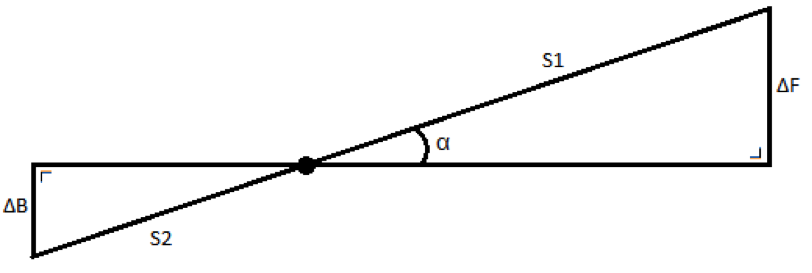
\includegraphics[scale=0.5]{figures/kantelpunt_launcher.png}
    \end{center}
    \caption{Schematische weergave servo montage punt.}
    \label{fig:berrLauncher}
\end{figure}

Door gebruik te maken van de bovenstaande formule is het mogelijk om de minimale montage hoogte van de
launcher te bepalen:

$\delta/B = S_2 \sin\alpha$

Bij het maken van deze berekening is het belangrijk rekening te houden met het bevestigingspunt
P zodat de servo niet te veel kracht moet zetten (dus niet te dicht bij het scharnierpunt). Daarnaast
is het belangrijk wel een goede hoek/actieradius te hebben. Dit is afhankelijk van de kijkhoek
van de camera en op welke afstand het systeem mensen moet kunnen herkennen/raken.

\subsubsection{Camera}
\label{subsub:camera}
De camera komt boven op het lanceer station zodat de software het gekleurde object kan detecteren en
de motor vervolgens naar dat punt in het beeld kan bewegen.

\subsubsection{Pan platform}
\label{subsub:panPlatform}
Het pan platform is enkel voorzien van een montage houder voor de tilt servo en
voetjes voor de montage van het lanceer platform.
Bij het ontwerp van dit platform moet rekening gehouden worden met het zwaartepunt. Dit
moet zo ver mogelijk in het midden van de pan servo liggen om een stabiel systeem te krijgen. Omdat
het zwaarte punt constant veranderd door het aantal Nerf darts en tilt hoek nemen we het
midden van de ‘launcher’ als zwaartepunt. Dan zal de tilt servo ongeveer op het tilt punt komen te
zitten.

\subsubsection{Basisstation}
\label{subsub:base}
Het laatste onderdeel is het platform waarin de pan servo wordt gemonteerd en de aansturing. Het
basisstation moet een goede constructie voor de pan servo geven zodat deze stabiel
kan bewegen. Daarnaast wordt op de achterkant de aansturing bevestigd. Het is belangrijk dat de
nodige beveiligingssystemen die op de aansturing zitten eenvoudig te bedienen zijn. De aansturing
wordt dan ook bij voorkeur achter het lanceer systeem en buiten het bereik van het pan platform.